\newcommand{\duedate}{17 September 2026}
\documentclass{16384_doc}
\usepackage{enumitem}
\usepackage{tikz}
\usetikzlibrary{positioning,arrows,arrows.meta,matrix,fit,backgrounds,calc,math,patterns,patterns.meta,intersections,fpu}
\newcommand{\assignmentname}{Assignment 5: Dynamics}

\begin{document}
\maketitle

\tableofcontents

\section{Theory Questions}

\begin{questions}
    \titledquestion{Spring, cart, pendulum}[30]

    The following spring-cart-pendulum system shown below is a modification of the pendulum-cart discussed in class. The cart has mass $M$, the pendulum has mass $m$ and its spring has rest length $r_0$ and spring constant $k$.
    \begin{center}
        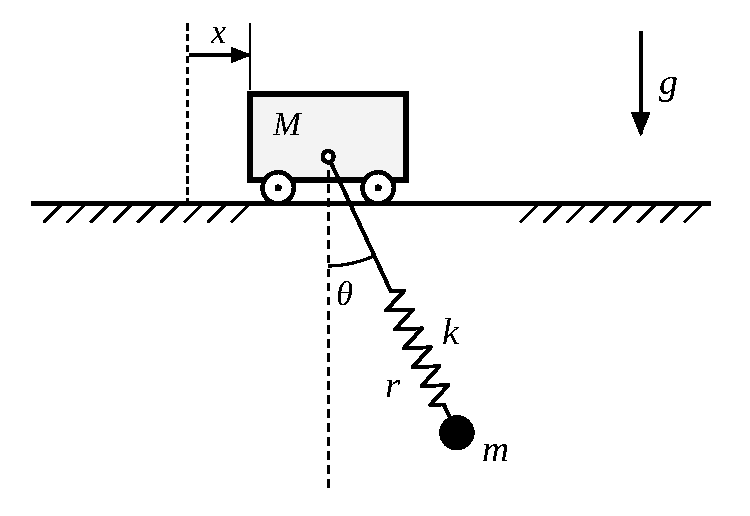
\includegraphics[width=0.4\textwidth]{generated_figures/cart_pendulum_spring.pdf}
    \end{center}

    \begin{enumerate}[label=\alph*.]
        \item \text{[10 points]} Write the potential and kinetic energy of the system in terms of the generalized coordinates $q = [x, r, \theta]^\top$ and their time derivatives $\dot q = [\dot x, \dot r, \dot\theta]^\top$. Then write the Lagrangian of the system.
        \begin{tcolorbox}[height=4cm]
            % TODO: ENTER YOUR ANSWER HERE
        \end{tcolorbox}

        \item \text{[10 points]} Write the derivatives of $\mathcal L$ with respect to $q$ and $\dot q$ (6 in total).
        \begin{tcolorbox}[height=6cm]
            % TODO: ENTER YOUR ANSWER HERE
        \end{tcolorbox}

        \pagebreak
        \item \text{[5 points]} Write the equations of motion of the system using the Euler-Lagrange equations.
        \begin{tcolorbox}[height=3cm]
        \end{tcolorbox}

        \item \text{[5 points]} Suppose you can control the cart with an external force $f_x$. Write the equations of motion with the control input $f_x$.
        \begin{tcolorbox}[height=3cm]
        \end{tcolorbox}
    \end{enumerate}

    \pagebreak
    \titledquestion{Double Pendulum}[30]
    The double pendulum is a classic example of a chaotic system, yet its equations of motion are relatively simple to derive. You will be using your derived equations of motion to simulate the double pendulum in the coding section of this assignment.

    The masses $m_1$ and $m_2$ are point masses at the ends of massless rods of length $\ell_1$ and $\ell_2$. Both angles are measured from the downward vertical, as shown in the figure: $\theta_2$ is the absolute angle of link 2, \emph{not} its angle relative to link 1. Gravity points in the $-y$ direction.

    \begin{center}
        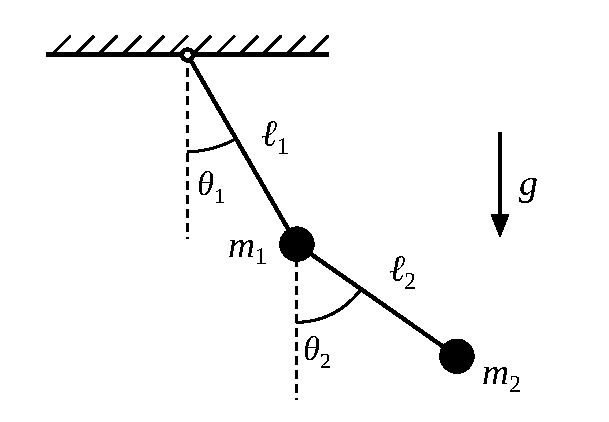
\includegraphics[width=0.4\textwidth]{generated_figures/double_pendulum.pdf}
    \end{center}
    
    \begin{enumerate}[label=\alph*.]
        \item \text{[10 points]} Write the potential and kinetic energy of the system in terms of the generalized coordinates $q = [\theta_1, \theta_2]^\top$ and their time derivatives $\dot q = [\dot \theta_1, \dot \theta_2]^\top$.
        \begin{tcolorbox}[height=4cm]
        \end{tcolorbox}

        \item \text{[10 points]} Write the derivatives of $\mathcal L$ with respect to $q$ and $\dot q$ (4 in total).
        \begin{tcolorbox}[height=6cm]
        \end{tcolorbox}

        \pagebreak
        \item \text{[10 points]} Write the equations of motion of the system using the Euler-Lagrange equations.
        \begin{tcolorbox}[height=3cm]
        \end{tcolorbox}
    \end{enumerate}

    \pagebreak
    \titledquestion{RR Arm Dynamics}[40]

    Consider the following robot. Assume no joint limits, and that the links lengths are $l_1=l_2=1$, and the masses are $m_1=m_2=1$. The joint angles are measured as a relative angle from the previous link / horizontal, so $\th[1]=\th[2]=0$ means the arm is fully extended to the right. Each link's mass is spread uniformly along its length, so its center of mass is at its midpoint and its moment of inertia about its center of mass is $I_i = \frac{1}{12} m_i l_i^2 = \frac{1}{12}$. Gravity points in the $-y$ direction.
    \begin{center}
        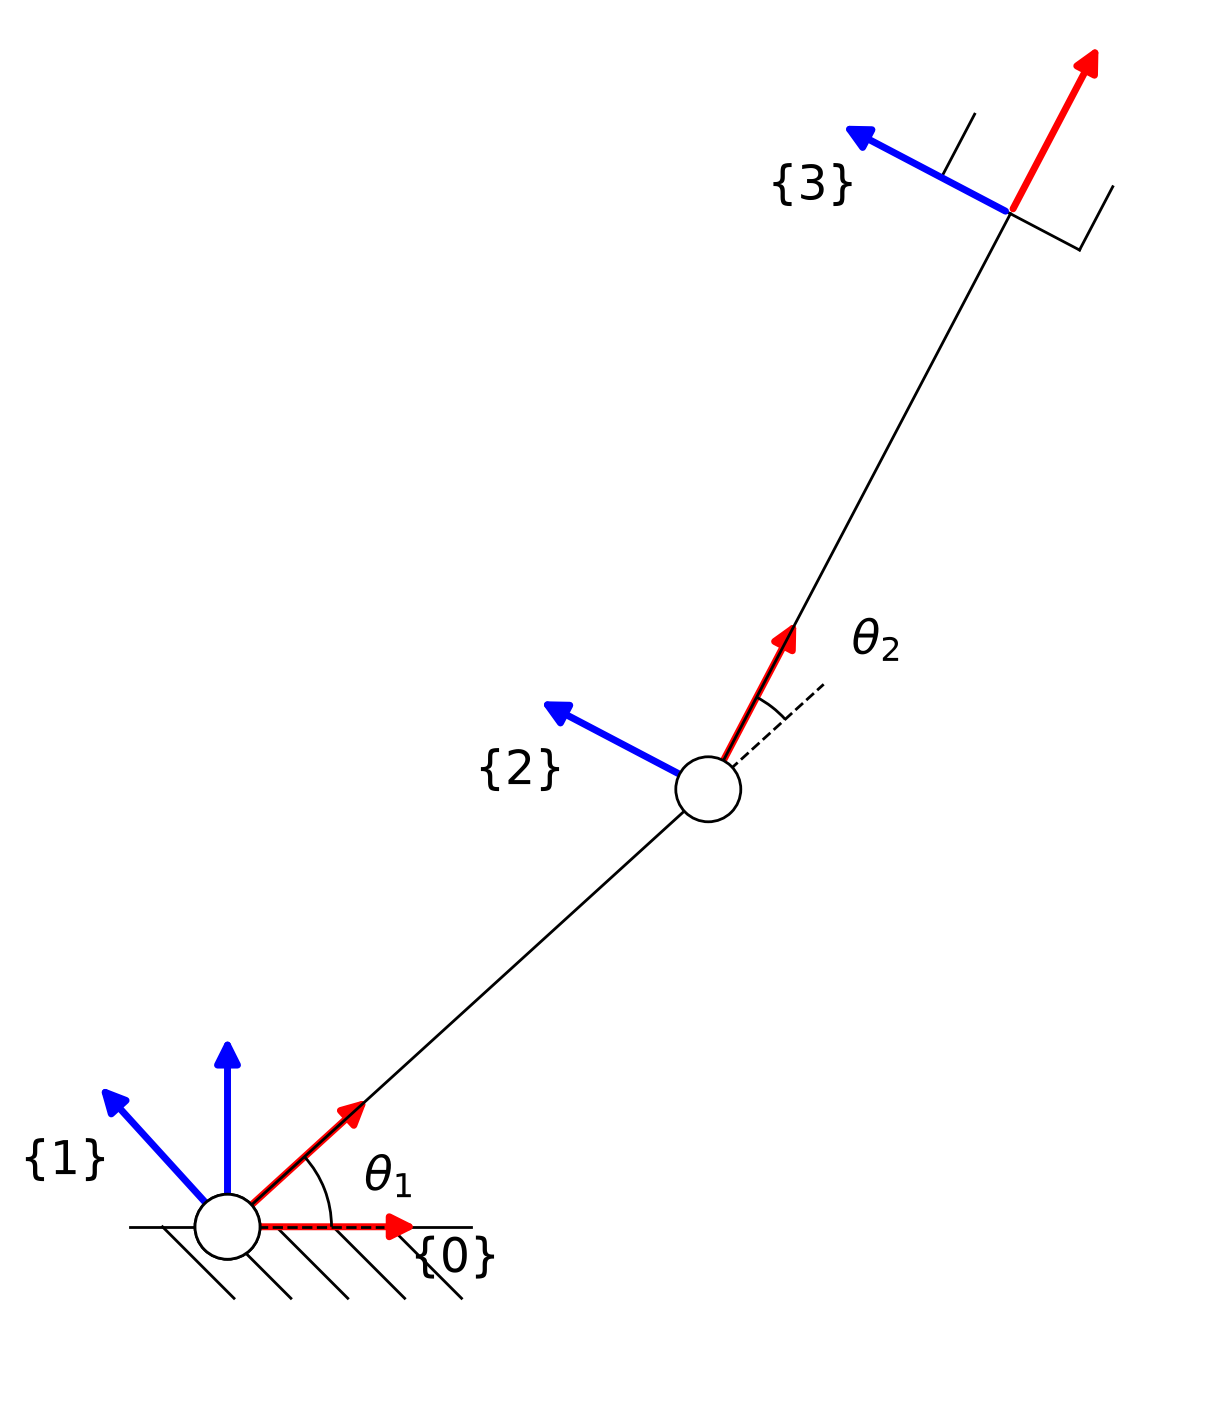
\includegraphics[width=0.4\textwidth]{generated_figures/robot_2.png}
    \end{center}

    \begin{enumerate}[label=\alph*.]
        \item \text{[10 points]} Write the potential and kinetic energy of the system in terms of the generalized coordinates $q = [\theta_1, \theta_2]^\top$ and their time derivatives $\dot q = [\dot \theta_1, \dot \theta_2]^\top$.
        \begin{tcolorbox}[height=4cm]
        \end{tcolorbox}

        \pagebreak
        \item \text{[10 points]} Write the derivatives of $\mathcal L$ with respect to $q$ and $\dot q$ (4 in total).
        \begin{tcolorbox}[height=6cm]
        \end{tcolorbox}

        \item \text{[10 points]} Write the equations of motion of the system using the Euler-Lagrange equations. Include external torques $\tau_1, \tau_2$ applied at each joint.
        \begin{tcolorbox}[height=3cm]
        \end{tcolorbox}

        \item \text{[5 points]} Find the standard form matrices $M(q)$, $C(q, \dot q)$, and $G(q)$ such that the equations of motion can be written as $M(q)\ddot q + C(q, \dot q)\dot q + G(q) = \tau$.
        \begin{tcolorbox}[height=3cm]
        \end{tcolorbox}

        \item \text{[5 points]} What are the joint torques $\tau_1, \tau_2$ required to hold the arm in the configuration $\theta_1 = \theta_2 = 0$ (fully extended to the right) with no motion? How does this compare to the Jacobian-based gravity compensation method discussed previously?
        \begin{tcolorbox}[height=3cm]
        \end{tcolorbox}
    \end{enumerate}


\end{questions}

\begin{submissionChecklist}
        \item Create a PDF of your answers to the written questions with the name \verb!<andrew_id>.pdf! and submit it to Gradescope.
\end{submissionChecklist}

\end{document}
